\documentclass[a4paper,12pt]{article}
\usepackage[brazil]{babel}
\usepackage[utf8]{inputenc}
\usepackage{indentfirst}
\usepackage{amsmath}
\usepackage{amsthm}
\usepackage{graphicx}
\usepackage{float}
\usepackage{array}
\usepackage[font=footnotesize,labelfont=bf]{caption}
\usepackage{geometry}
\usepackage{listings}
\usepackage{subcaption}
\usepackage{xcolor}
\usepackage{float}
\usepackage[skins,xparse,breakable]{tcolorbox}
\usepackage{longtable}
\usepackage{minted}
\usepackage{graphicx}
\usepackage{enumitem}
\usepackage{geometry}
\usepackage{titlesec}
\usepackage{fancyhdr}

\geometry{left=2.5cm, right=2.5cm, top=3cm, bottom=3cm}

% Cabeçalho e rodapé
\pagestyle{fancy}
\fancyhf{}
\lhead{Proposta de Projeto TP1 - Tonhão Autopeças}
\rhead{Grupo 08 - UnB}
\cfoot{\thepage}

% Configuração das seções
\titleformat{\section}{\bfseries\Large}{\thesection.}{1em}{}
\titleformat{\subsection}{\bfseries\normalsize}{\thesubsection.}{1em}{}

\begin{document}

\begin{center}
  \textbf{\Huge Proposta de Projeto TP1\\ Tonhão Autopeças} \\[0.5em]
  Nirva Neves de Macedo, 232009585\\
  Henrique Morcelles Salum, 232003008\\
  Dérick Daniel Silva de Andrade, 231003522\\[0.5em]
  Departamento de Ciência da Computação – Universidade de Brasília (UnB)\\
  CIC0197 – Técnicas de Programação 1 – Grupo 08\\
  \texttt{232009585@aluno.unb.br, 232003008@aluno.unb.br, 231003522@aluno.unb.br}
\end{center}

\begin{abstract}
Este documento apresenta a proposta de trabalho do grupo 08 para a disciplina de Técnicas de Programação 1, Turma 03, semestre 2024/2. Serão abordadas as ideias iniciais e preliminares para a realização do projeto, bem como o diagrama de classes associado.
\end{abstract}

\section{Introdução}

Oficinas mecânicas são essenciais para a manutenção da infraestrutura centrada em carros no Brasil. Infelizmente, são normalmente conhecidas por suas baixas confiabilidades e desorganização, especialmente quando estão afastadas de polos urbanos.

Visando uma solução moderna e simples para essas instituições, propomos um software de gerenciamento baseado em classes, com o objetivo de fornecer uma interface objetiva para gerenciar os seguintes elementos:

\begin{itemize}[noitemsep]
    \item Clientes
    \item Carros
    \item Estoque de peças
    \item Ordens de serviço
\end{itemize}

O sistema atribui as ordens de serviço ao cliente, carro e funcionário respectivos, provendo status de conclusão, status de pagamento e método de pagamento. Ele também gerencia o estoque ao solicitar novas peças e deduzir peças usadas em um serviço. O sistema automatiza a demanda de peças, verificando a disponibilidade no estoque e alocando-as automaticamente ao serviço solicitado.

\section{Regras de Negócio}

\begin{itemize}[noitemsep]
    \item Clientes que pagarem em dinheiro ou Pix recebem 5\% de desconto.
    \item A cada R\$2.000,00 pagos, o cliente ganha um check-up completo do veículo e troca de óleo gratuitos.
    \item Funcionalidades de cadastrar, alterar e excluir objetos do programa requerem login de administrador.
\end{itemize}

\section{Divisão de Tarefas}

O relatório correspondente a cada classe e tela é de responsabilidade do membro que a desenvolveu.

\begin{itemize}[noitemsep]
    \item \textbf{Dérick}:
    \begin{itemize}[noitemsep]
        \item Classes: Pessoa, Cliente e Funcionário.
        \item Telas: Cadastro de pessoas e tela de login.
    \end{itemize}
    \item \textbf{Henrique}:
    \begin{itemize}[noitemsep]
        \item Classes: Veículo e Serviço.
        \item Telas: Cadastro de veículos e gerenciamento de serviços.
    \end{itemize}
    \item \textbf{Nirva}:
    \begin{itemize}[noitemsep]
        \item Classes: Estoque e Peça.
        \item Telas: Tela inicial, estoque e cadastro de peças.
    \end{itemize}
\end{itemize}

\section{Diagrama de Classes}

% Substitua pelo caminho correto da imagem
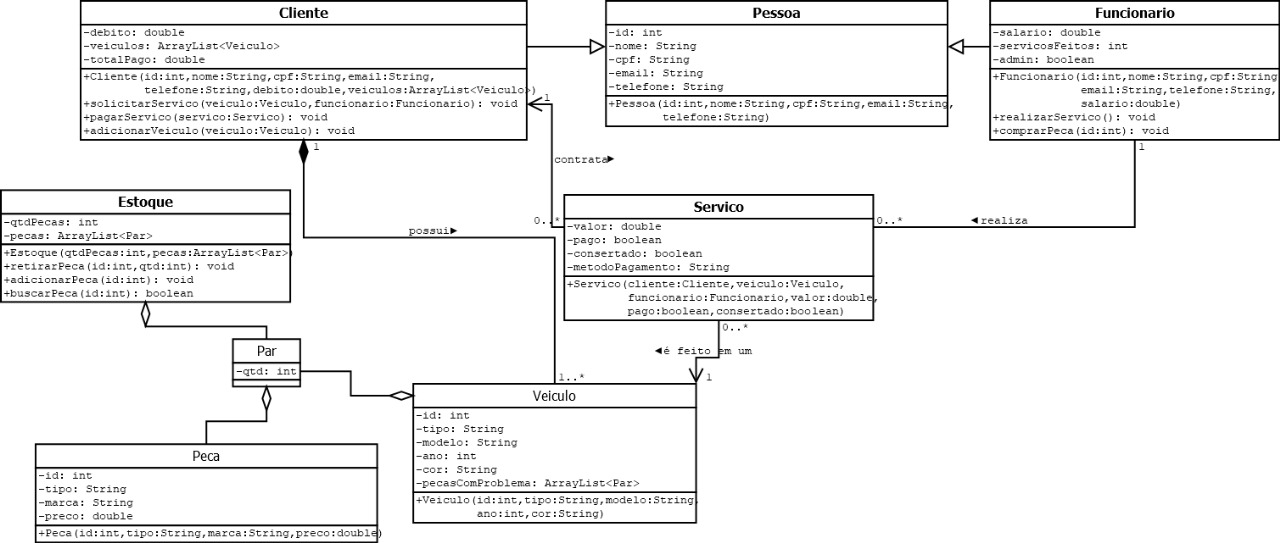
\includegraphics[width=\textwidth]{imagens/diagrama_de_classes.jpg}

\end{document}
